% !TeX root = document.tex
% !TeX encoding = UTF-8 Unicode

\chapter{Resultados e Discussões}%
\label{chp:results}

Neste capítulo são apresentados os resultados parciais obtidos, separados por
tópicos conforme o cronograma apresentado na proposta.

\section{Estudos teóricos}%
\label{sec:studies}

\subsection{Controle preditivo por modelo}%
\label{subsec:mpc-studies}

O livro-texto utilizado para os estudos do controle preditivo por modelo foi o
do~\textcite{book:wang}, com as outras referências sendo usadas de forma
complementar. Para a execução deste projeto propõe-se o estudo dos capítulos 1 a
4, que tratam do caso discreto.

Foram estudados os capítulos 1 e 2, que apresentam o conceito do controlador e a
formulação com restrições, respectivamente. Como os estudos teóricos de \ac{MPC}
foram iniciados antes da alteração da eletrônica do forno, a técnica foi testada
utilizando os tanques comunicantes (Figura~\ref{fig:tanks}) presentes no
Laboratório de Sinais e Sistemas.

\begin{figure}[ht!]
    \centering
    \captionsetup{justification=centering}
    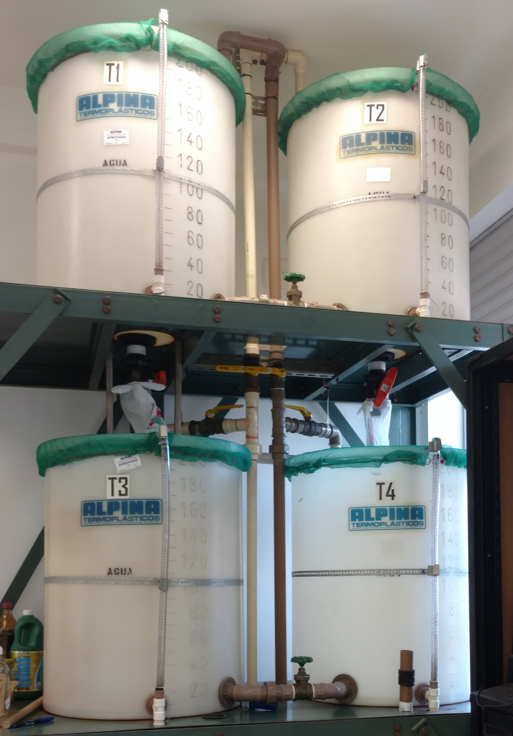
\includegraphics[height=0.5\linewidth]{imgs/tanques}
    \caption{Sistema de tanques comunicantes}%
    \label{fig:tanks}
\end{figure}

Os tanques utilizados são o 1º e 2º, que estão localizados na parte superior e
marcados como T1 e T2. A bomba insere água no primeiro tanque e esta escoa para
o segundo através de uma válvula localizada na parte inferior. A água é então
removida através de uma válvula no fundo do tanque 2. O objetivo de controle é
o nível do tanque 2.

Uma simulação do controlador MPC controlando o modelo desse sistema pode ser
visto na Figura~\ref{fig:mpc-simulated}. Observa-se que o sinal de controle é
mantido em 100\% por quase todo o transitório, e é então abaixado para o valor
de equilíbrio, fazendo com que o tanque encha de forma rápida mas minimizando o
overshoot.

\begin{figure}[ht!]
    \centering
    \captionsetup{justification=centering}
    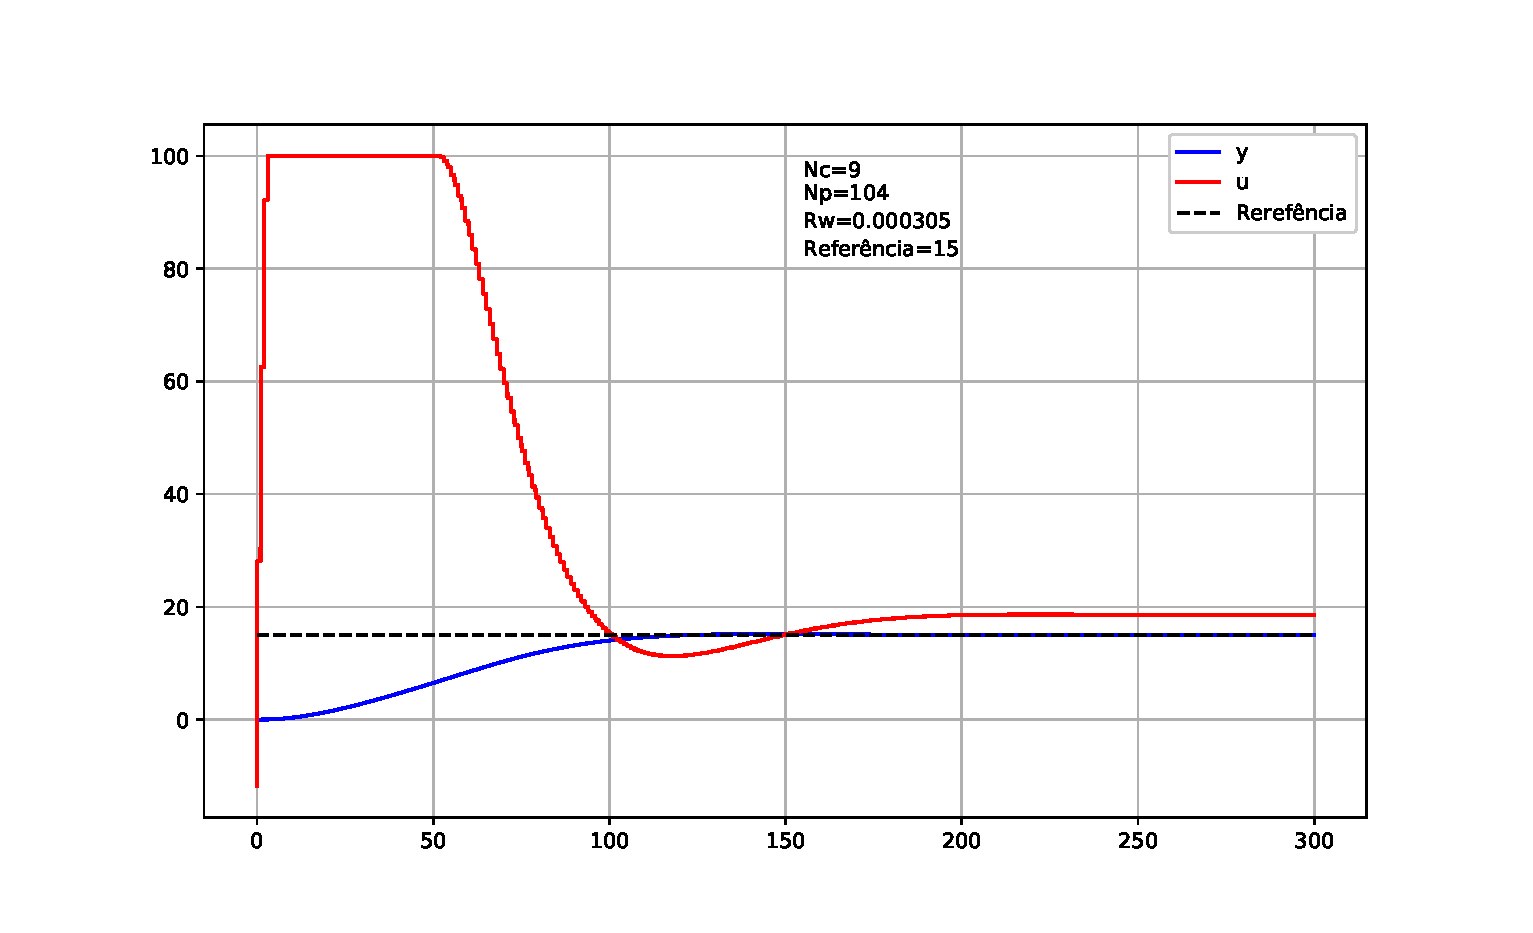
\includegraphics[height=0.5\linewidth]{imgs/mpc-simulado}
    \caption{Simulação do modelo dos tanques com controlador MPC}%
    \label{fig:mpc-simulated}
\end{figure}

Ao inserir este controlador no sistema real (Figura~\ref{fig:mpc-tanks})
obtem-se uma resposta parecida com a da simulação, porém mais lenta. Essa
diferença pode ser explicada por erro de modelagem e pelo fato que o sistema
real não é linear, sendo o modelo linearizado. No entanto a resposta continua
satisfatória.

\begin{figure}[ht!]
    \centering
    \captionsetup{justification=centering}
    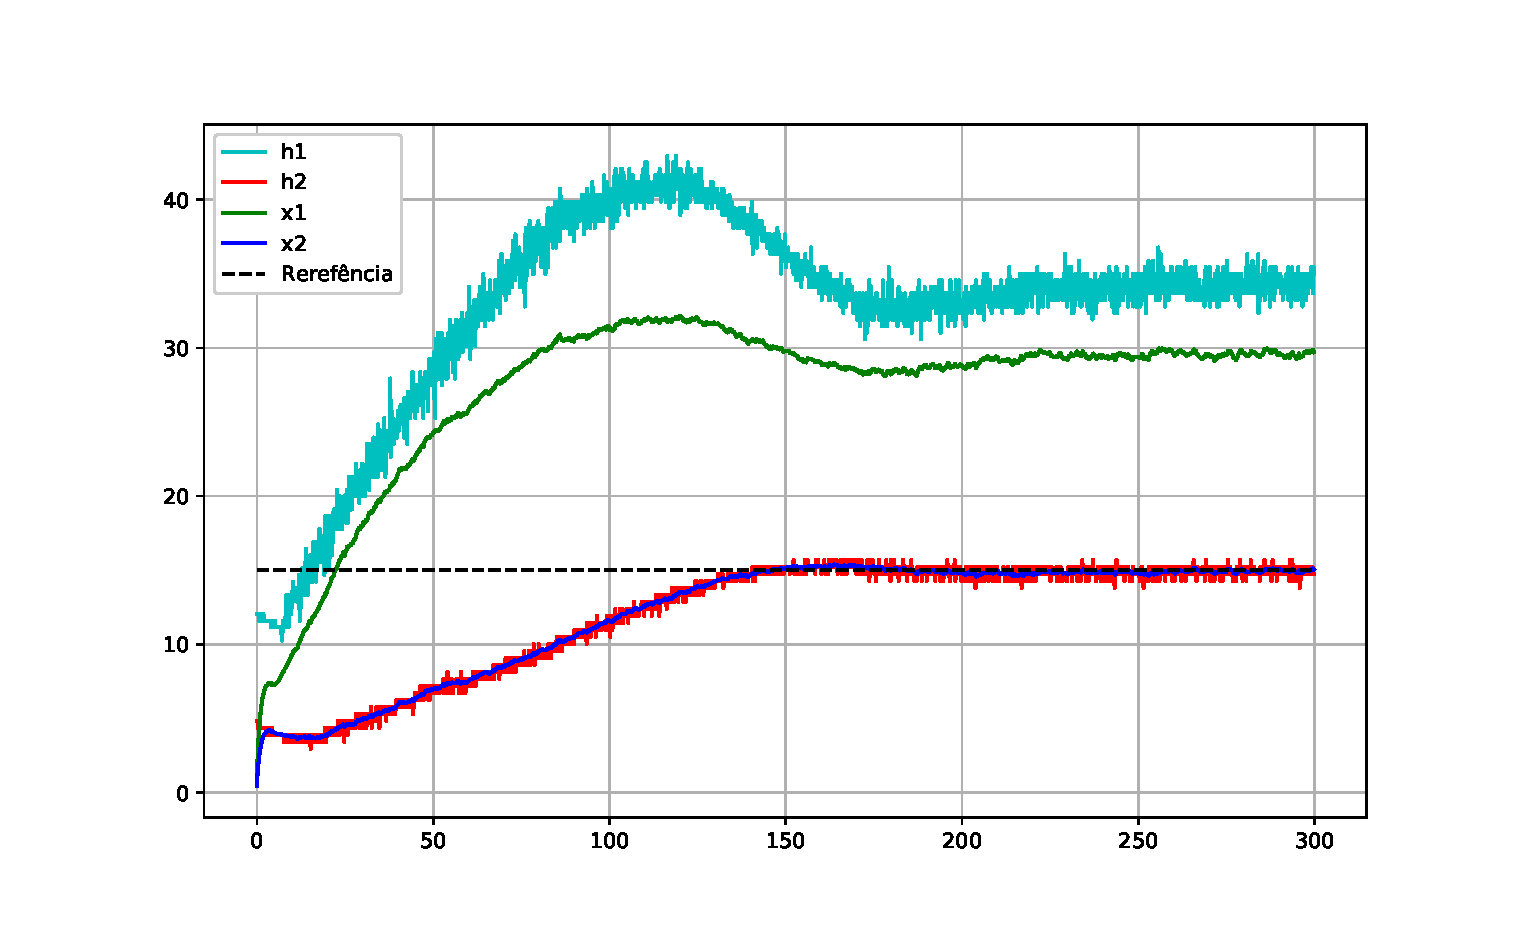
\includegraphics[height=0.5\linewidth]{imgs/mpc-tanque}
    \caption{MPC aplicado ao sistema real}%
    \label{fig:mpc-tanks}
\end{figure}

Como foi utilizado um observador, também pode-se perceber os efeitos do erro de
modelagem. Os estado estimado, \( x_1 \), embora apresente a mesma dinâmica, não
apresenta o mesmo ganho que o estado real, \( h_1 \). É interessante notar, no
entanto, que esta diferença não atrapalha o controlador, que continua capaz de
seguir a referência.

\subsection{Modelagem térmica e SPD}%
\label{subsec:spd-studies}

Os resultados obtidos por~\textcite{masterthesis:nelson} foram simulados e
utilizou-se o modelo \ac{SPD} apresentado com os observadores de Kalman e
exponencial com fator de esquecimento. Foi possível ver nos estados a saída
variando conforme a distância do atuador aumenta, como pode ser visto na
Figura~\ref{fig:spd-sim}. Os observadores também estimam com precisão os estados
do sistema simulado, conforme Figura~\ref{fig:spd-obs}.

\begin{figure}[ht!]
    \centering
    \captionsetup{justification=centering}
    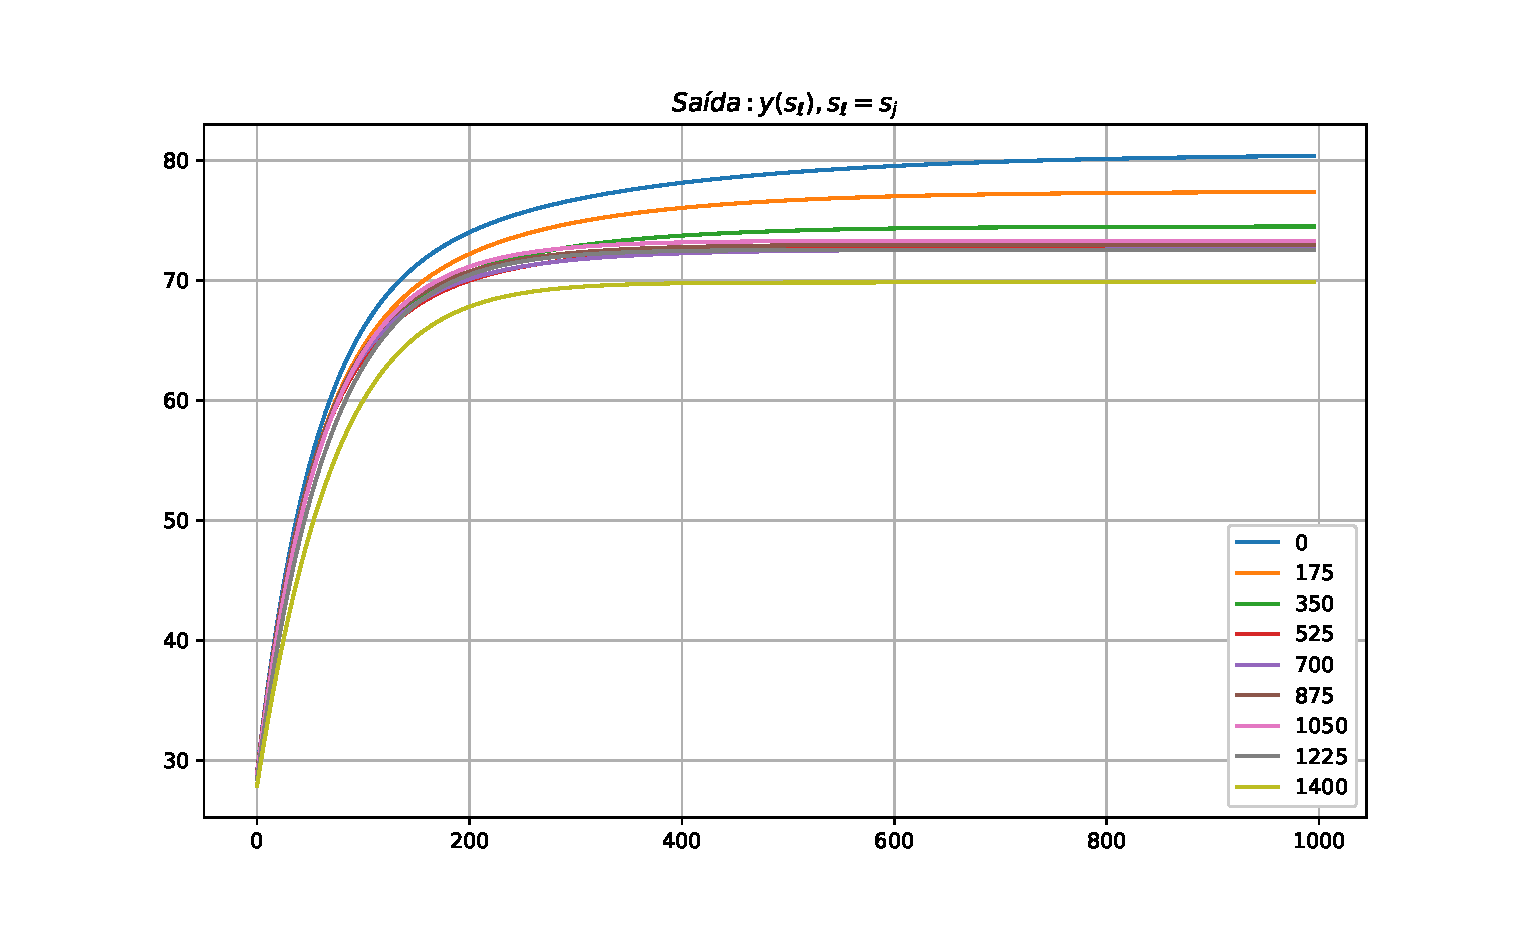
\includegraphics[height=0.5\linewidth]{imgs/spd-sim}
    \caption{SPD simulado}%
    \label{fig:spd-sim}
\end{figure}

\begin{figure}[ht!]
    \centering
    \captionsetup{justification=centering}
    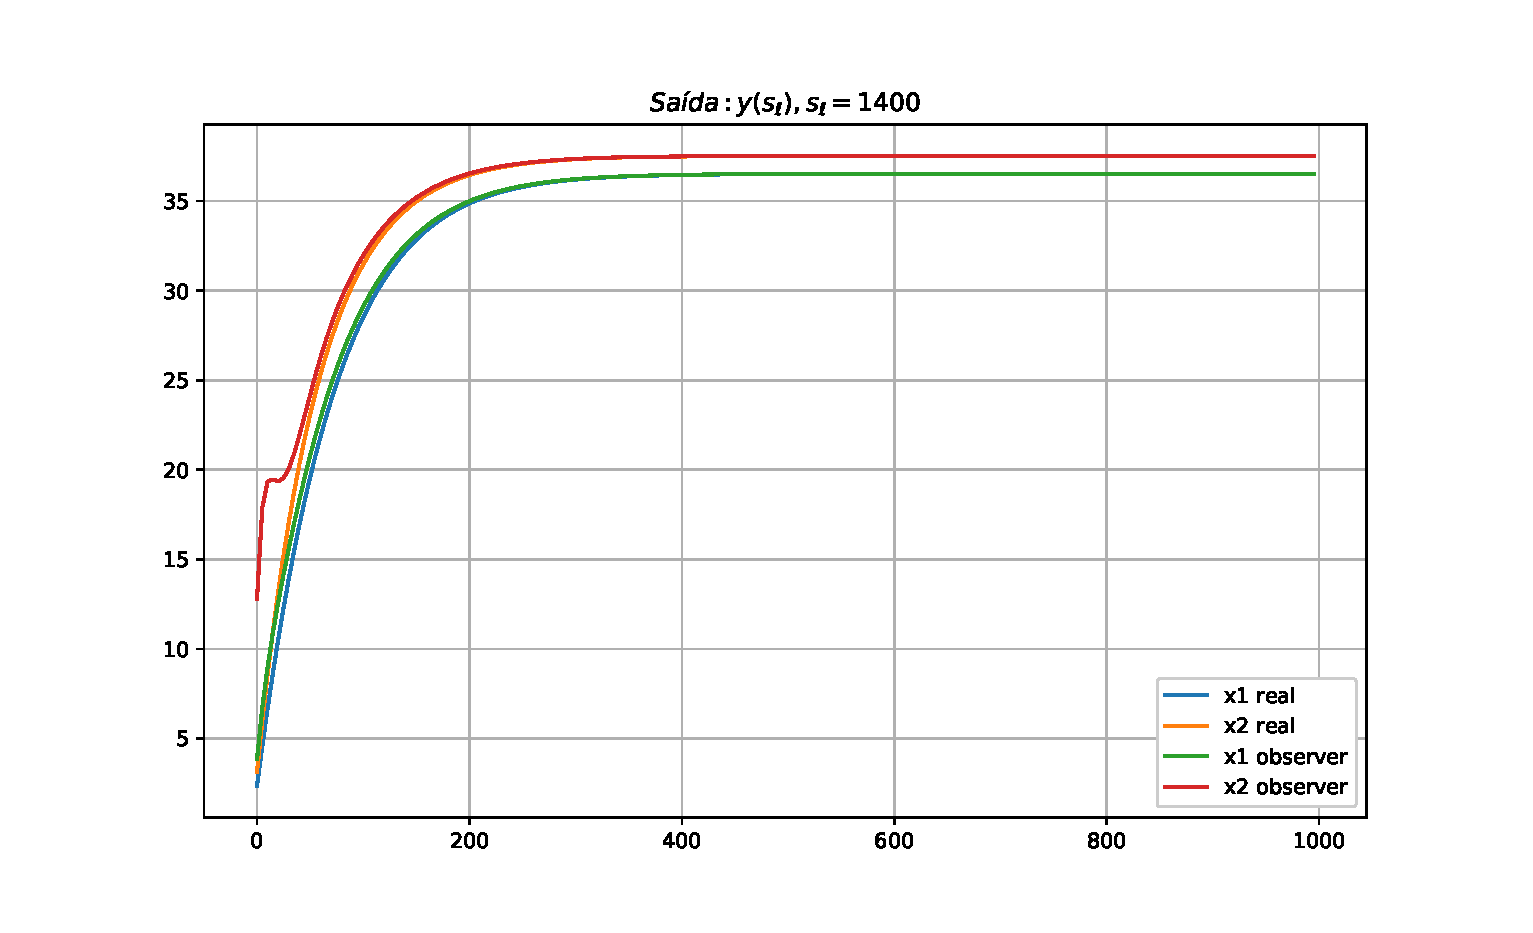
\includegraphics[height=0.5\linewidth]{imgs/spd-obs}
    \caption{SPD simulado com observador exponencial}%
    \label{fig:spd-obs}
\end{figure}

\section{Modificação do hardware e implantação da plataforma}%
\label{sec:hardware-and-plataform}

Ao estudar o circuito de acionamento e sensoriamento percebeu-se que não há a
necessidade de alterar o circuito. Devido a forma como o mesmo está montado, foi
necessário apenas a reprogramação dos microcontroladores presentes para
possibilitar a comunicação direta através de cabos USB.\ Após a reprogramação
foi possível acionar o circuito de potência e ler os valores dos sensores.

A instalação do Raspberry não foi feita pois o mesmo não foi adquirido a tempo.
No entanto, as modificações necessárias para a sua inserção já foram executadas
em outros projetos. Tais modificações compreendem principalmente mudanças no
software \textit{moirai} e já foram publicadas.

\section{Calibrações, testes e certificações}%
\label{sec:calibration}

O funcionamento do circuito eletrônico foi feito primeiramente acionando o
sistema desenvolvido por~\textcite{masterthesis:nelson}. Após verificar que este
era capaz de acionar as resistências e ler valores de todos os sensores, foi
feita a modificação dos códigos dos microcontroladores para permitir a
comunicação com a plataforma e testou-se novamente com o novo código.
Verificou-se a necessidade de recalibrar os sensores e reordená-los,
identificando qual estava conectado a qual porta. Devido a forma como se dá o
acionamento não é necessária a calibração dos atuadores.

Para a calibração dos sensores foi utilizada uma garrafa térmica perfurada e uma
lâmpada incandescente. A mesma foi ligada e foram feitas medições das
temperaturas dos sensores bem como de um termômetro industrial a cada 10
segundos. Foram coletados 160 pontos. Utilizou-se então a técnica do mínimos
quadrados para encontrar uma expressão de correção linear, \( ax+b \), cujos
coeficientes podem ser vistos na Tabela~\ref{tbl:calib-coefs}.

\begin{table}[ht!]
    \centering
    \caption{Coeficientes da calibração}%
    \label{tbl:calib-coefs}
    \begin{tabular}{ccccccccccc}
          & S1    & S2   & S3   & S4   & S5   & S6   & S7   & S8   & S9   & S10  \\
        a & 0.85  & 0.82 & 0.82 & 0.78 & 0.79 & 0.83 & 0.76 & 0.74 & 0.81 & 0.79 \\
        b & -0.65 & 3.32 & 3.40 & 3.06 & 4.96 & 2.12 & 5.24 & 6.21 & 1.39 & 4.55
    \end{tabular}
\end{table}

A validação dos modelos e observadores ainda está sendo executada, pois foram
encontradas dificuldades durante a validação. O problema encontrado é que o
observador não está estimando o segundo estado corretamente. O proponente
buscará resolver este problema juntamente com seu orientador e o author do
modelo.

\section{Melhorias na plataforma}%
\label{sec:platform-enhancements}

Foram feitas várias modificações na plataforma. A lista completa pode ser vista
nos \textit{commits} de cada projeto, publicados desde 1º de março de 2018:

\begin{itemize}
    \item Lachesis: \url{https://github.com/acristoffers/Lachesis/commits/master}
    \item moirai: \url{https://github.com/acristoffers/moirai/commits/master}
    \item ahio: \url{https://github.com/acristoffers/ahio/commits/master}
\end{itemize}

As modificações que se destacam são:

\begin{itemize}
    \item implementação de um mecanismo de \textit{backup} de todo o banco: o
          uso de múltiplos computadores na mesma planta pode ser facilitado com
          a opção de realizar backup de todo o banco. Isso também permite a
          liberação de espaço no sistema sem a perda de dados, já que pode-se
          guardar os dados antigos e apagar os testes, deixando a interface mais
          limpa;
    \item implementação de imporatação e exportação de configuração de hardware:
          também interessante quando várias pessoas utilizam o mesmo hardware.
          Mudanças, como novas calibrações, podem ser compartilhadas de forma
          simples e novos usuários podem começar a utilizar a planta
          rapidamente, apenas importando uma configuração já testada;
    \item seleção das variáveis a serem exibidas em gráficos: durante o
          desenvolvimento inicial não se pensou na possibilidade do usuário
          precisar salvar dezenas ou centenas de variáveis. Toda variável salva
          geraria um gráfico para o usuário, sempre. Durante os testes com casos
          reais, realizados por alunos de graduação e mestrado, observou-se a
          necessidade de limitar o número de gráficos gerados sem limitar o
          número de variáveis salvas. Isso foi feito colocando uma opção de
          selecionar quais gráficos serão exibidos;
    \item opção de clonar um teste ou controlador: durante os testes também
          percebeu-se a necessidade de duplicar um teste inteiro para modificar
          apenas um valor de variável, ou outra modificação pequena;
    \item melhoria da forma de apresentação de erros no terminal: os erros
          apresentados no terminal não eram explicativos, não mostrando, por
          exemplo, onde ocorreu o erro. Agora os erros trazem o escopo e a linha
          do erro, bem como a mensagem principal (erro mais relevante). Esse
          erro, na versão 1.0.11 do Lachesis, também é exibido para o usuário na
          interface, no componente Gráficos;
    \item melhoria de velocidade na recuperação de dados do banco: foram
          utilizadas funções disponíveis em versões mais recentes do MongoDB
          para melhorar a filtragem e transformação dos dados retornados. Esses
          eram feitos anteriormente em Python, com uma implementação mais lenta
          que aquela do banco de dados;
    \item inserção de um novo banco de dados: MySQL (necessário no Raspberry),
          sua necessidade veio da modificação anterior. Ao atualizar o banco de
          dados percebeu-se que as versões mais novas não mais suportam sistemas
          operacionais de 32bits, por isso foi necessário encontrar um banco de
          dados capaz de executar em um Raspberry Pi de 32bits. A seleção do
          MySQL se deu pela sua disponibilidade e atualização no Raspbian,
          sistema operacional do Raspberry e por sua implementação em linguagem
          C/C++. Outros bancos de dados não estruturados do tipo
          \textit{document store} foram considerados, mas a falta de
          documentação, api pobre e/ou implementação em linguagem interpretada
          (mesmo que por máquina virtual) os fizeram menos interessantes;
    \item implementação de busca por drivers (ahio) em caminhos arbitrários: a
          biblioteca ahio implementa alguns drivers padrão que estão presentes
          em seu código fonte. No entanto, faz-se necessário a implementação de
          drivers específicos, que não devem ser inseridos e distribuídos na
          biblioteca por não serem úteis em outros contextos, por exemplo, o
          driver do forno e os drivers utilizados pelos alunos Affonso Salomão e
          Bernardo Amin em seus TCCs. Para solucionar esse problema criou-se a
          possibilidade de procurar por drivers em caminhos informados pelo
          usuário, exportando-se funções para adicionar e remover caminhos do
          \textit{PATH}. No aplicativo \textit{moirai} foi criada a opção de se
          definir uma variável de ambiente denominada \textit{AHIO\_PATH}
          contendo caminhos separados por \enquote{:} (dois pontos), conforme
          padrão \textit{POSIX}.
\end{itemize}
